\section{Evaluation}
\label{sec:eval}

\subsection{Methodology}
\label{sec:eval-method}

We run on a two-vCPU container with 4\,GiB of RAM and CPython 3.11; the host is
deliberately small, so absolute latencies are a conservative upper bound. Experiments
use three seeds and report the mean, except the cap sweep, which is rerun on twelve;
per-seed rows ship with the code.

The generator produces $12{,}000$ requests from $40$ tenants over $1{,}500$
subjects and three platforms, with popularity from a truncated Zipf law of exponent
$1.15$ and $15\%$ of requests touching several subjects; every subject carries a cap
of $\eps{=}1.0$ at $\delta=10^{-5}$. Identities are drawn by inverse transform, so
large ranks fold back onto small ones and the heavy hitters that make accounting hard
survive.
The splitting attack gives an adversary $12$ target subjects, a budget of
$0.30\eps$ per target and $k$ fragments from $12$ to $60$, issued under distinct
identities across platforms.

We compare against five policies: \emph{static quota}, a fixed per-platform
allowance that meters spend but can neither throttle nor window it; \emph{token
bucket}, a per-subject allowance that refills at $0.05\eps$ per second; \emph{audit only}, which admits everything and
flags subjects afterwards and is the deployed status quo; \emph{exact blocking},
per-platform counters checked against composed spend; and \emph{exact global}, exact
per-subject counters shared across tenants and platforms, with no window, breaker or
degradation. \sys\ is the only
policy that is subject-keyed across platforms, time-structured and memory-bounded in
its estimator.

\subsection{Is the Estimator Sound and Accurate?}
\label{sec:eval-accuracy}

A false negative in the estimate cannot release an over-cap answer, because the
ledger refuses it; what an under-estimate costs is a late throttle, which is why
the estimator is built one-sided. Across 24 configurations---four widths, with and
without the hot table, three seeds---the estimate never falls below the true charge,
as Proposition~\ref{prop:onesided} requires, including across eviction and
re-admission.

The monitor, not the estimator, limits what the SLO means (E25). At 24 checkpoints of
a 600\,s trace at cap 0.5 we recompute the exact windowed composition of every subject
and compare it with the rate the hot table reports. In the heavy-tailed population the
table's recall is 1.0 for $H\ge64$ and 0.66--0.95 at $H{=}8$, and the monitored rate matches
the population rate to three decimals. Flatten the popularity
(Zipf 0.6) and shrink the table to eight slots and recall collapses to 0.014: 70 of 71
violations are missed, and the monitored rate reads 0.000 against a population rate of
0.002, because violators are no longer heavy hitters. Scanning the sketch over all $N$
subjects recovers every violation in both regimes with at most two false alarms in
1{,}500 subjects---the loss is sampling, not conservatism---but the scan costs $O(N)$
per epoch. The windowed SLO is therefore best effort over the population; the cap is
not.

Accuracy separates along the population. For the top percentile by spend---the
subjects whose budgets bind---relative error is 4.3\% without a hot table at width 512
and 0.02\% from width 2048 up, where the table rather than the width does the work. For
the tail, mean absolute error falls from 0.071$\eps$ to 0.013 and p99 from 0.37 to 0.10;
width 32{,}768 measures zero error, which is why we do not deploy it.

\subsection{What Does It Cost?}
\label{sec:eval-cost}

The estimator costs 27--32\,$\mu$s per request across widths from $2^{10}$ to
$2^{16}$, against 4.6\,$\mu$s for an exact table: an 18\% rise for a sixteen-fold
increase in width, as expected from eight memory accesses per update plus the hot-table
lookup. The full admission path is slower and far more variable
(Fig.~\ref{fig:latency}a). Its tail came from one function: a tenant-pressure sweep
that scanned the hot table every 64 admissions, which cost p99 5.8\,ms against
0.9\,ms with the sweep removed. We replaced it with an incremental update at commit
time---$O(\text{ring})$ per charge, and a monitor over every charged subject rather
than the hot table---and the p99 falls to 1.1\,ms for the same trace and host, with
the mean moving from 0.28 to 0.23\,ms (E17).

Queueing still decides the deployment (Fig.~\ref{fig:latency}b): at 50\%
utilisation the median is 0.26\,ms but the p99 is 160\,ms; a load that averages
50\% while peaking at five times capacity makes the median 0.9\,s. The path must be
provisioned for its peak, and microsecond averages are the wrong number to quote.

Memory tells the opposite story at small scale: below roughly $10^{4}$ subjects a
dense table is no larger than the sketch, because the sketch's width is paid once and
the table's cost has not caught up (Fig.~\ref{fig:scale}). From $10^{3}$ to $10^{6}$
subjects the dense table grows from 1.2\,MB to 1.2\,GB while the sketch stays at
10.6\,MB (E23); per-request cost rises from 25 to 45\,$\mu$s for the sketch and 9 to
13\,$\mu$s for the table, and the estimate keeps its one-sidedness, with maximum
absolute error 0.057$\eps$ (E8).

\begin{figure}[t]
\centering
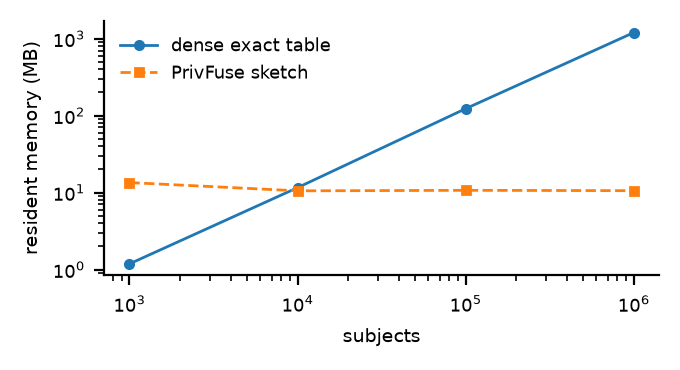
\includegraphics[width=0.88\columnwidth]{figures/fig7_scale.png}
\caption{Resident memory as the subject population grows (E23), with the default
four live tables. The dense table grows linearly with $N$; the sketch is flat. Zero
under-estimates at every population.}
\label{fig:scale}
\end{figure}

\begin{figure}[t]
\centering
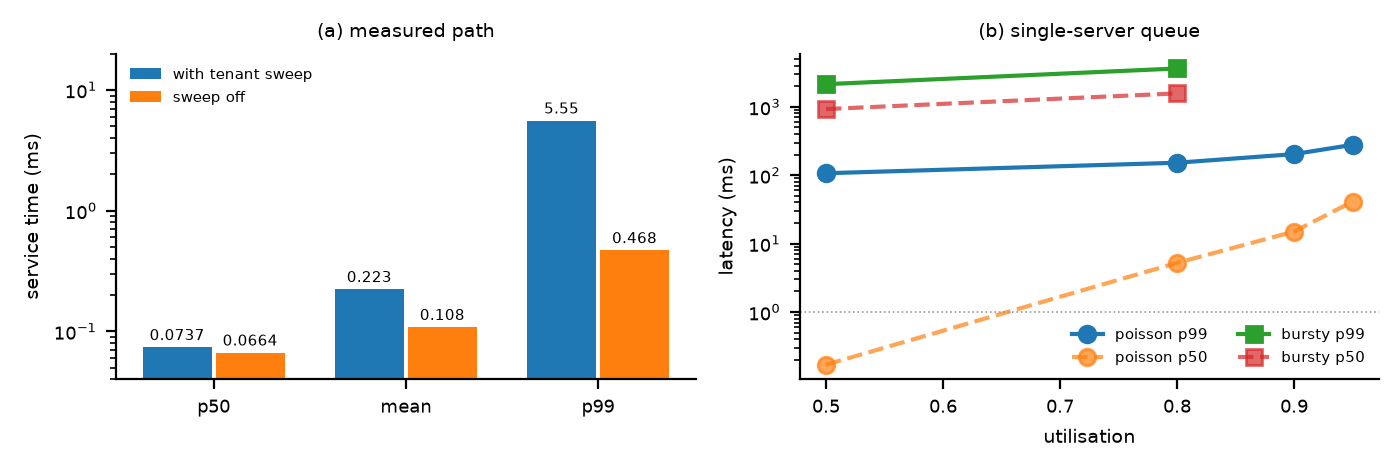
\includegraphics[width=0.9\columnwidth]{figures/fig17_latency.png}
\caption{Admission latency (E17, 12{,}000 requests, median of three trials). (a)
Service time under the per-request pressure sweep and under the incremental monitor we
adopt, log scale. (b) FCFS queue over the measured service times under Poisson arrivals
and under a burst at five times the average rate.}
\label{fig:latency}
\end{figure}


The structure answering windowed queries is therefore $O(1)$ in $N$, whereas a
naive windowed accountant---one cumulative structure per epoch---multiplies the
measured 1.2\,GB by the ring depth. The whole system is not: the ledger keeps one
scalar balance per subject that has ever transacted, far smaller than a cost vector,
and a deployment would shard it.
